%    Template for seminar reports
% Seminar Current Topics in Computer Vision and Machine Learning
% Summer Semester 2015
% Computer Vision Group, Visual Computing Institute, RWTH Aachen

\documentclass[twoside,a4paper,article]{combine}


% =========================================================================
\usepackage[utf8]{inputenc}
%\usepackage[ngerman]{babel}
\usepackage{a4}
\usepackage{fancyhdr}   
%\usepackage{german}    % Uncomment this iff you're writing the report in German
\usepackage{makeidx}
\usepackage{color}
\usepackage{t1enc}		% german letters in the "\hyphenation" - command
\usepackage{latexsym}	% math symbols
\usepackage{amssymb}    % AMS symbol fonts for LaTeX.
\usepackage{amsmath}

\usepackage{graphicx}
\usepackage{pslatex}
\usepackage{ifthen}

\usepackage[T1]{fontenc}
\usepackage{pslatex}

\usepackage{psfrag}
\usepackage{subfigure}
\usepackage{wrapfig}
\usepackage{url}

% =========================================================================

\setlength{\oddsidemargin}{3.6pt}
\setlength{\evensidemargin}{22.6pt}
\setlength{\textwidth}{426.8pt}
\setlength{\textheight}{654.4pt}
\setlength{\headsep}{18pt}
\setlength{\headheight}{15pt}
\setlength{\topmargin}{-41.7pt}
\setlength{\topskip}{10pt}
\setlength{\footskip}{42pt}

\setlength{\parindent}{0pt}

% =========================================================================

\graphicspath{
	{img/}
}

%%%
% We want also subsubsections to be enumerated
%%%
\setcounter{secnumdepth}{3}
\setcounter{tocdepth}{3}

\makeglossary
%\makeindex

% =========================================================================
\begin{document}

% Template for seminar reports
% Seminar Current Topics in Computer Vision and Machine Learning

\begin{titlepage}


\begin{center}
\ 
\vspace{3.5cm}


\textsf
{
Fakultät für Mathematik, Informatik und Naturwissenschaften\\
Lehr- und Forschungsgebiet Informatik VIII\\
Computer Vision\\
Prof. Dr. Bastian Leibe
}

\rule{\linewidth}{1pt}

\vspace{1.75cm}
\LARGE
\textbf{Seminar Report}

\vspace{1.7cm}
\huge
Combining 3D Shape, Color, and Motion for Robust Anytime Tracking

\vspace{3.0cm}
\Large
Frederik Zwilling\\
\large
Matriculation Number: 304314

\vspace{0.5cm}
June 2015

\vspace{1.05cm}
\rule{\linewidth}{1pt}

\vspace{0.5cm}
\textsf{\textbf{
\normalsize
\begin{tabular}{ll}
Advisor:  & Aljoša Ošep\\
\end{tabular}
}}
\end{center}

\end{titlepage}


\begin{abstract}
  \textcolor{red}{Abstract}
\end{abstract}

\tableofcontents
\newpage
% =========================================================================

\section{Introduction}
\label{sec:intro}
Robust and precise position and velocity estimation is an important
part of object tracking. For example, it is an essential part in the collision
avoidance of an autonomous car. This report presents a
method by Held, Levinson, Thrun, and Savarese to solve this part of
the tracking problem by combining clues of the 3D shape, color and motion of
the tracked object~\cite{paper}. The method uses a probabilistic
measurement model derived from a Dynamic Bayesian Network. The search
space, consisting of position and velocity, for each tracked object is represented
in a special dynamic histogram, called \textit{annealed dynamic
  histogram}. This histogram dynamically increases its resolution in
the important areas and considers the local resolution in the
measurement model. By expanding the measurement model with color and motion the
performance of the method can be further improved. This is shown by the authors
by evaluating in a static environment, where only the reference system
is moving, and in a dynamic environment, where the compactness of the
models build with the tracking results is used as evaluation criteria. 


\subsection{Motivation}
\label{sub:motivation}
Robotic applications are about to change many domains from the ground
up. Especially autonomous systems could take over dangerous,
exhausting and unpopular tasks and thus allow humans to do more satisfying
tasks instead. Additionally, autonomous systems can be more efficient
and scalable than solving the tasks by hand. Some progressive domains
with autonomous robots are flying drones, which can map
areas~\cite{auto-drones} or deliver
packages~\cite{auto-delivery-drones}, autonomous cars, which take care
of driving~\cite{auto-cars}, logistic robots, which store and grab
goods in warehouses~\cite{kiva}, and domestic service robots, which
can support old people and clean at home~\cite{athome}. All these
domains have in common that the robots have to track objects in their
environment, mostly for avoiding collisions. In the case of domestic
service robots, tracking is also needed for follow people. Often the reliability
and precision of the tracking are limiting factors. An autonomous car,
for example, can only drive fast if it is sure that it
tracks all objects in the surrounding correctly and none of these
objects could cause a collision. This report mainly focuses on the
domain of autonomous cars. Here, the autonomous system takes care of
the time consuming driving task on the one hand and could help to
reduce the amount of traffic deaths ($25,938$ in $2013$ in the
EU~\cite{traffic-deaths}) on the other hand. In this domain it is
especially important to estimate the speed of various nearby objects
robustly and in real time. Figure~\ref{fig:objects} shows the three
main classes of objects that have to be tracked, cars, bicycles, and
pedestrians, in challenging situations. The method proposed in this
report solves this task and performs better than previous approaches
in the car domain.
\begin{figure}
  \subfigure[Cars on a highway]{%
    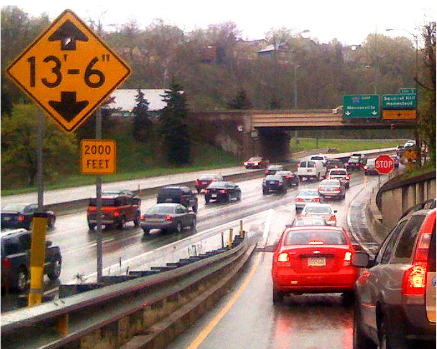
\includegraphics[height=.3\linewidth]{highway}
  }
  \subfigure[A cyclist]{%
    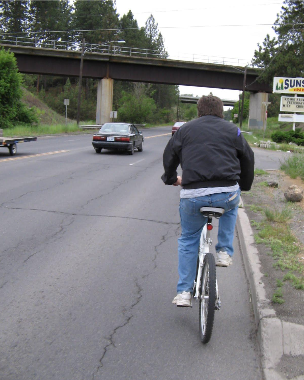
\includegraphics[height=.3\linewidth]{bicycle}
  }
  \subfigure[A pedestrian]{%
    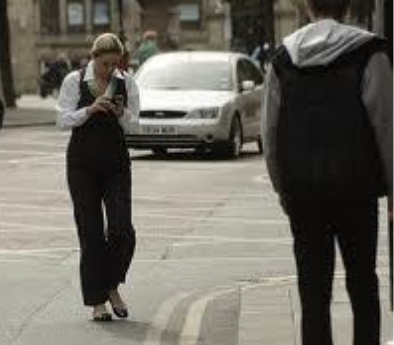
\includegraphics[height=.3\linewidth]{pedestrian}
  }
  
  \caption{Various objects that have to be tracked in challenging
    situations~\cite{held-website}}
  \label{fig:objects}
\end{figure}


\subsection{Tracking}
\label{sub:tracking}
Object tracking is the complex task to identify objects and their
movement over time. It can be separated into the following parts. The
first step segments the sensor data for time $t$, called
\textit{frame}, into detected objects. This can be done for example by
separating foreground and background and find connected components in
the foreground. In this step, it is beneficial to use the information that
the most important objects to find are cars, bicycles and
pedestrians~\cite{segmentation}. The second step is to associate
detected object in the successive frames $t$ and $t+1$. One method to
find these matchings is to compute descriptors, such as the HOG
descriptor, for the objects and find nearest neighbors in the
descriptor space~\cite{arbitrary-object-recognition}. The third step
is the position and velocity estimation of the tracked object. That is
the part of tracking this report is about. In the forth step, the
computed trajectory of the tracked object is classified to decide, for
example, if the object is dangerous to the car.

The data that is used for tracking in this report is generated by a
dense laser sensor that measures the distance to surrounding objects
with multiple rotating laser beams. Such a sensor and the data
generated by it is shown in Figure~\ref{fig:lidar}. Additionally, the
sensor provides a camera image similar to a panorama.
\begin{figure}
  \center
  \subfigure[]{%
    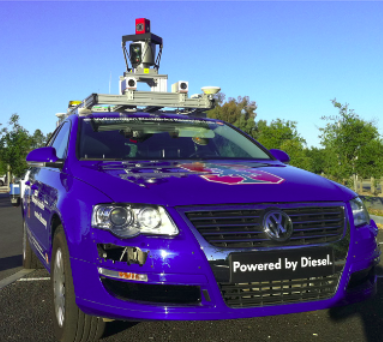
\includegraphics[height=.35\linewidth]{lidar}
  }
  \subfigure[]{%
    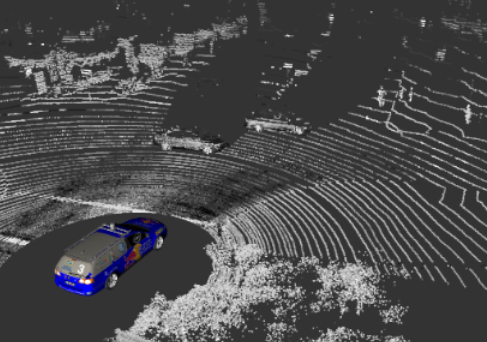
\includegraphics[height=.35\linewidth]{lidar-data}
  }
  
  \caption{A Velodyne LIDAR sensor mounted on a car (a) and a
    visualization of the point cloud generated by it
    (b)~\cite{arbitrary-object-recognition}.}
  \label{fig:lidar}
\end{figure}

\subsection{Velocity and Pose Estimation}
\label{sub:vel-and-pos-estimation}
To compute the pose and velocity estimation of an object, we first
introduce a measurement model that is derived from a Dynamic Bayesian
Network (\textit{DBN}). This DBN models for each frame the
dependencies between position, velocity, object surface and the
observed measurement as well as the dependencies between two
frames. Though, tracking is a hard
problem because in cases with occlusion and major changes in the
viewpoint the visible object surface can differ significantly and
introduce an error. Especially in these cases, it is intuitive to also
consider color and motion in the measurement model because the additional
information is influenced less by occlusion and viewpoint changes.

To find the state, which is composed of position and velocity of an
object, we use a histogram that maps the each histogram-chunk in the
state space to the probability that this chunk causes the measurement
according to our model. This allows a global search in the state space
with multiple hypothesis. A standard histogram with adequate
resolution would have to many chunks and thus would be to slow for
real time computation. Therefore, we use a dynamic histogram that
starts with a low resolution and an approximated posterior
distribution. Then it dynamically increases the resolution in areas
with high probability to cause the measurement. This allows to achieve
a result after running the method for any time. The downside of the
dynamic histogram is that the initial low resolution introduces an
additional error. This can be balanced by including the resolution in
the measurement model. We call this method \textit{annealed dynamic
  histogram} because as the resolution increases, the distribution is
annealed and approaches the true posterior.

The evaluation in Section~\ref{sec:evaluation} shows that the method
outperforms other tracking methods by about $10\%$.
\textcolor{red}{Maybe add more evaluation intro?}

% +++++++++++++++++++++++++
\section{Related Work}
\label{sec:related-work}
The tracking problem has been studied for many years. The most common
approaches to estimate the position and velocity of tracked objects,
namely Kalman filters and Iterative Closest Point,
are described in subsection~\ref{sub:pos-vel-est-alt}. Often these
approaches are efficient but sacrifice a lot of the available data by
using simple representations or search only for a local maximum.
Because
our case of tracking objects in 3D point clouds from a laser sensor is
only a special case of tracking,
subsection~\ref{sub:slternative-sensors} gives an overview of the
tracking approaches with other sensors, mainly single cameras and
stereo cameras.
Subsection~\ref{sub:grid-based-methods} presents
grid-based approaches that are similar to annealed dynamic histograms.

\subsection{Position and velocity estimation alternatives}
\label{sub:pos-vel-est-alt}
Some simple approaches to estimate position and velocity of a tracked
object first represent the object by its
centroid~\cite{kalman-centroid, towards-aut-cars} or bounding
box~\cite{kalman-bounding-box, kalman-bounding-box2,
  kalman-bounding-box3} and then use a Kalman
filter~\cite{ai-modern}. This is a computationally efficient approach
but discards a lot of available information by using such a simple
representation. Therefore, this approach is especially fragile in cases
of occlusion and viewpoint changes. In the occlusion case, the
bounding box can contain only a part of the object and the centroid
would be shifted. In the viewpoint-change case, the centroid and
bounding box can significantly differ (e.g. when seeing a cyclist from
the back and the side). Another disadvantage of the Kalman filter is
that it can only represent a single hypothesis and thus performs
poorly when multiple hypotheses are reasonable.

Other approaches include domain specific knowledge to use better
fitting object representations. For example, the typical shape of a car
with its corners or wheels can be use to achieve a more precise
position of a car in a frame~\cite{use-car-shape, use-car-shape2,
  use-car-shape3}. This leads to better detection and association
results, but is limited by the amount of trained
object-classes. Although cars, pedestrians and cyclists are the most
common classes, it is also important to detect uncommon obstacles in
traffic (e.g. tractors, segways, and wheelchairs). The work presented
in this report is based on~\cite{arbitrary-object-recognition}. It
allows recognition and classification of arbitrary objects and only
requires labeled dataset to train the object-classes. Another approach
that can track known objects as well as fully unknown objects
is~\cite{leibe-tracking-before-detection}. This approach differs from
the previous ones by performing the tracking before the detection
step what enables it to track unknown objects.

A widely used alternative to Kalman filters is the Iterative Closest
Point (ICP) algorithm~\cite{icp, icp2,
  leibe-tracking-before-detection}.
The algorithm merges
two point clouds by finding a maximum correspondence
alignment. Thus the full 3D point cloud is used. It
uses a hill climbing approach and therefore depends on a good
initialization and can get stuck in a local maximum. This is the major
drawback of ICP and has a large impact on the tracking precision as
shown by~\cite{icp-bad, icp-bad2}. Figure~\ref{fig:icp} visualizes how
ICP can return a wrong alignment after an unlucky initialization.
\begin{figure}
  \center
  \subfigure[Bad initial alignment]{%
    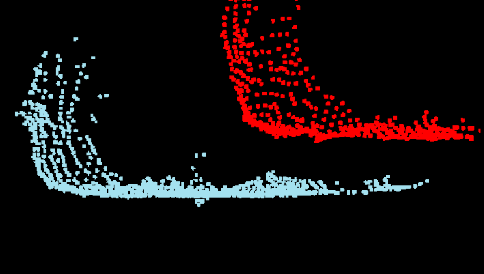
\includegraphics[height=.28\linewidth]{icp-init}
  }
  \subfigure[Stuck in a local maximum after 3 iterations
  (green arrows)]{%
    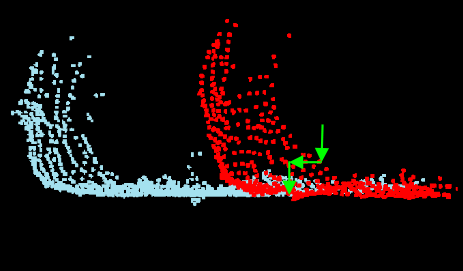
\includegraphics[height=.28\linewidth]{icp-stuck}
  }
  
  \caption{Possible case for bad ICP alignment results. The two point
    clouds belong a detected car in successive frames~\cite{held-website}.}
  \label{fig:icp}
\end{figure}
The approach presented in this report performs a global search and
therefore has no problem with local maxima.

\subsection{Alternative Sensors}
\label{sub:slternative-sensors}
Laser range sensors, such as the one shown in Figure~\ref{fig:lidar},
are not the only kind of sensors used for tracking tasks. Although
laser range sensors provide more precise data compared to other
sensors used for tracking, they are inadequate
for many applications because of their high price. A closely related
alternative to laser range sensors is the usage of stereo
cameras. They provide the same kind of data (point clouds and images)
and are cheap. However, they have more noise then a laser sensor and
can therefore cause larger errors in the tracing results. An example
for the use of stereo data for tracking
is~\cite{leibe-tracking-before-detection}. It uses ICP to track
pedestrians and unknown objects. Object tracking with a single camera
has been studied for a long time and is used in many applications,
e.g. in video calling~\cite{single-camera-tracking}. However, single
camera tracking is unsuitable in the autonomous car scenario because
of missing depth information.

\subsection{Grid-Based Methods}
\label{sub:grid-based-methods}
Ordinary grid-based search approaches in computer vision are used to
globally search in a state space and allow multiple hypothesis in
contrast to Kalman filters and ICP. However, the computational
effort increases with the resolution of the grid. Therefore,
ordinary histograms are often inadequate for domain which require
real time computation.
Dynamic histograms tackle this problem by starting with a low
resolution and increasing the resolution in important areas. However,
this creates the problem that the low resolution introduces an
additional error.

There already are some grid-based approaches which tackle this
problem. Most of them are used in Simultaneous Localization and
Mapping (\textit{SLAM}). \cite{multi-res-grid-slam2} uses a grid-based
Monte-Carlo method that recursively expands grid cells with the
most hypotheses and refines the grid resolution in these cells. This
only differs from annealed dynamic histograms in the usage of a
Monte-Carlo distribution instead of probabilities to cause the current
measurement. The approach presented in~\cite{multi-res-grid-slam}
self-localizes a robot with a dynamically refined grid. Here, each
measurement point votes for the cells that could have caused the
measurement. The cells with the most votes are refined in the next
iteration. Similarly to the paper presented in this report, the
approach enables anytime computation.

The main differences between previous methods and the method presented
in this report are the additional consideration of color, what is not
directly possible in Kalman filter or ICP approaches, and the
consideration of the probabilities for points being occluded in
previous frames. This leads to higher tracking
robustness. Furthermore, annealed dynamic histograms allow multiple
hypotheses and globally
searching the state space. In contrast to other
grid-based approaches, it also allows real-time computation without
introducing a high error resulting from low resolution by
annealing the measurement model as the resolution increases.

% +++++++++++++++++++++++++
\section{Method}
\label{sec:method}
The method presented in this report consists of three major
parts. Subsection~\ref{sub:probabilistic-model} introduces the
probabilistic model based on a Dynamic Bayesian Network. The model is
necessary to determine how likely it is that a specific position and
velocity of a detected object causes the observed
measurement. In Subsection~\ref{sub:adding-color} the extension of the
measurement model by color and motion is shown~\cite{paper}.
Subsection~\ref{sub:adh} describes how annealed dynamic
histograms are used to search the state space for the most likely
position and velocity according to the measurement model. For that
especially the refinement steps, that increase the resolution, and the
annealing of the measurement model depending on the resolution are
important.

\subsection{Probabilistic Model}
\label{sub:probabilistic-model}

\begin{figure}
  \center
  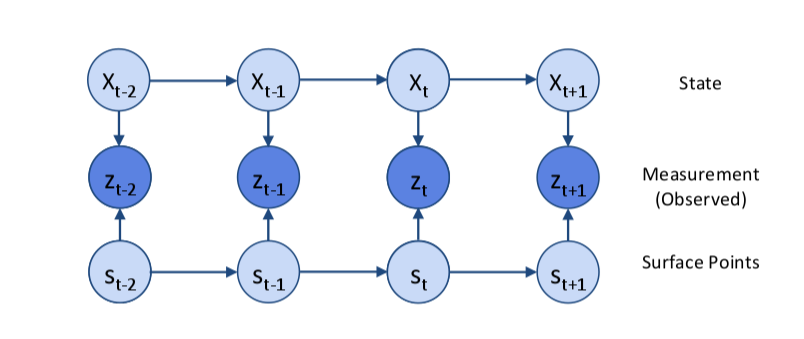
\includegraphics[width=.8\linewidth]{dbn}
  \caption{Dynamic Bayesian Network to derive the measurement model
    for tracking an object~\cite{paper}.}
  \label{fig:dbn}
\end{figure}

To derive the probability for a position and velocity to cause the
observed measurement seen in the last frames, we use a Bayesian
Network because it allows us to easily combine 3D shape, color, and
motion cues~\cite{paper}. After encoding the influences of the states,
consisting of position and velocity, the surface of the object to
track and the observed measurement, we can derive the wanted
probability of the measurement given the state by applying well known
probability rules in Bayesian Networks~\cite{ai-modern}. Furthermore,
we use a Dynamic Bayesian Network to relate variables over successive
time steps.

The Dynamic Bayesian Network we use to derive the measurement model is
shown in Figure~\ref{fig:dbn}. For the frames $t-2$ to the current
frame $t+1$, it includes the variables $x$ for the state, $z$ for the
observed measurement and $s$ for the visible surface of the object. In
the following, we describe these variables in detail.

As state variable $x_t$, we use the composition of position and
velocity $x_t=(x_{t,p},\dot{x}_{t,p})$. $x_{t,p}$ is the linear
position of the object centroid in frame $t$ relative to the centroid
of the object in frame $t-1$. In other words, the centroid of the
object in frame $t-1$ is the origin of the coordinate system for
$x_{t,p}$. $\dot{x}_{t,p}$ is the velocity of the object. The relative
rotation and the rotational velocity of the object is not included in
the state. This speeds up the method because a lower dimensional state
space is considered. The authors claim that omitting the rotation is
no problem because the rotational velocity of the objects present in
traffic is small relative to the frame rate of the sensor, which is
$10Hz$. Similarly, also the vertical movement of the objects is
small because the objects we are interested in move along the
ground. Therefore, we can use a 2D position and velocity instead of a
3D position and velocity. To use the methods in other domains that
require considering the vertical velocity, the state space can be
expanded, what results in a slow down of the method.
%Alternative elivation map?

To include the 3D shape of the object in the model we use the latent
surface variable $s_t$. It represents the visible surface of the
object and is a set of $n$ points $\{s_{t,1}, ..., s_{t,n}\} = s_t$
that are sampled from the visible surface. Although the true 3D shape
of the object is unknown and only indirectly observable through the
measurement, it is important for the model. This is similar to SLAM
methods which model the environment map that corresponds to the surface in our
terminology.The measurement then depends on the modeled map and the
\begin{wrapfigure}{r}{0.45\linewidth}
  \center
  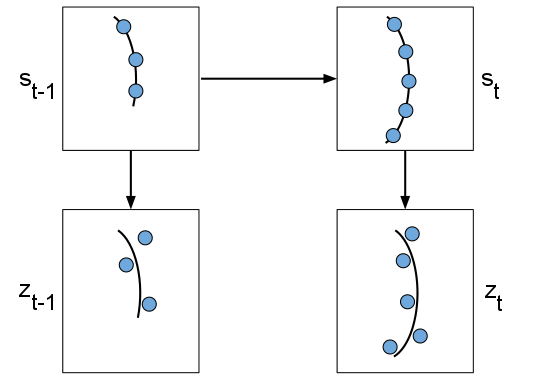
\includegraphics[width=\linewidth]{surface-measurement}
  \caption{Measurement points $z_t$ sampled with sensor noise
    $\Sigma_e$ from surface points $s_t$. The visible surface, from which the
    surface points are sampled, varies from frame to frame due to
    occlusion and viewpoint changes~\cite{paper}.}
  \label{fig:surface-measurement}
\end{wrapfigure}
localization, or the object surface and state in our case. When
looking at the Dynamic Bayesian Network in Figure~\ref{fig:dbn}, it is
easy to see that considering the surface is important because, when it
is omitted, two successive measurements would be independent given the
state variable. This would be wrong because the shape of the object is
relatively consistent and therefore also the measurement points
describe a similar surface. In contrast to SLAM, it is not our goal to
build the shape of the observed object. We simply integrate over
shapes to get the surface. The prior of the surface points
$p(s_{t,i})$ is a uniform distribution over the maximum size of an
object. The prior of the surface is the product over its points
$p(s_{t})=\Pi_i p(s_{t,i})$.
The observed measurement $z_t$ is again a set of measurement points
$z_t=\{z_{t,1}, ..., z_{t,m}\}$. These points depend on the latent
surface $s_t$ and the position $x_{t,p}$. However, the measurement
points do not lie directly on the surface as illustrated in
Figure~\ref{fig:surface-measurement}. This is caused by the sensor
noise, which depends on the sensor resolution and is modeled as
Gaussian noise $\Sigma_e$. The sensor resolution can roughly be modeled as a
linear function of the distance between object and sensor. The
generation of measurement points $z_t$ depending on the surface points
$s_t$, the sensor noise $\Sigma_e$ and the position $x_{t,p}$ can be written as
\begin{equation}
\label{eq:gaus-zt}
z_{t,i} \sim \mathcal{N}(s_{t,i},\Sigma_e) + x_{t,p} \mbox{ . }
\end{equation}
Because the origin of the coordinate system is placed at the centroid
of the object in the previous frame, the measurements of the previous
frame are not shifted
\begin{equation}
\label{eq:ind-centroid}
z_{t-1,i} \sim \mathcal{N}(s_{t-1,i},\Sigma_e) \mbox{ . }
\end{equation}
Therefore, $z_{t-1}$ is conditionally independent from $x_{t-1}$ what
is not derivable by just using the Bayesian Network in
Figure~\ref{fig:dbn}.

For the derivation of the measurement model, we will also need the
term $p(s_t|s_{t-1})$ which stands for the probability of sampling
surface points $s_t$ from the currently visible surface given
$s_{t-1}$ from the previous frame. The sampled points might differ
because of occlusions, viewpoint changes, random sampling from the
surface and deformations of the object (e.g. body movement of a
walking pedestrian). Every point of $s_t$ could have been generated
from a visible or occluded part of the surface in frame $t-1$. When we
consider the prior probability $p(V)$ for sampling from a previously
visible surface, we can use the joint distribution over these two
cases:
\begin{align}
\label{eq:st-st-1}
p(s_{t,i}|s_{t-1})=&p(V)*p(s_{t,i}|s_{t-1},V) + \nonumber\\
&p(\neg V)*p(s_{t,i}|s_{t-1},\neg V)
\end{align}
$p(s_{t,i}|s_{t-1},\neg V)$ stands for the probability that $s_{t,i}$
is generated from a part of the surface that was not visible in the
previous frame. Under the assumption that every non visible point is
occluded, we can rewrite the term with constants $k_1$ and $k_2$:
\begin{equation}
p(s_{t,i}|s_{t-1},\neg V) = k_1 (k_2 - p(s_{t,i}|s_{t-1},V))
\end{equation}
This allows simplifying Equation~\ref{eq:st-st-1} to
\begin{equation}
\label{eq:prob-surf}
p(s_{t,i}|s_{t-1})=\eta_1 (p(s_{t,i}|s_{t-1},V) + k)
\end{equation}
with the normalization constant $\eta_1=p(V)-p(\neg V) k_1$ and the
smoothing factor $k=p(\neg V)k_1k_2/\eta_1$.
%Possible equation
These constants can later be found by training.

$p(s_{t,i}|s_{t-1},V)$ can be modeled by a
Gaussian distribution
\begin{equation}
\label{eq:gaus-st-i}
s_{t,i} \sim \mathcal{N}(s_{t-1,j},\Sigma_r)
\end{equation}
where $s_{t-1,j}$ is the closest corresponding surface point from the
previous frame and $\Sigma_r$ is the variance mainly resulting from
the sensor resolution and the object deformation. Combining these
Gaussians in Equation~\ref{eq:prob-surf} for all surface points in
$s_t$ yields
\begin{equation}
\label{eq:gaus-st}
p(s_{t}|s_{t-1}) = \eta(\mathcal{N}(s_t;s_{t-1,i},\Sigma_r) + k) \mathrm{ . }
\end{equation}

For the measurement model used in the annealed dynamic histogram, we
need to derive $p(z_t|x_t,z_1,...,z_{t-1})$, the probability for the
current measurement given the histogram cell with state $x_t$ and the
previous measurement history $z_1$ to $z_{t-1}$. Though considering all
previous measurements of the object would be computationally
costly. Although the measurements in different time frames are not
independent given the state, as discussed earlier, we can focus only
on the previous one as approximation, because the previous one has the
highest impact of all measurements in the history.
\begin{equation}
p(z_t|x_t,z_1,...,z_{t-1}) \approx p(z_t|x_t,z_{t-1})
\end{equation}
This approximation can be rewritten by using the joint distribution over
all surface points in the current and previous frame:
\begin{equation}
\label{eq:mm-iint}
p(z_t|x_t,z_{t-1}) = \iint p(z_t,s_t,s_{t-1}|x_t,z_{t-1}) \mathrm d
s_t \mathrm d s_{t-1}
\end{equation}
Because of the chain rule of probabilities and the conditional
independences that could be derived from the Dynamic Bayesian Network
in Figure~\ref{fig:dbn}, we can refine the term in the integral:
\begin{align}
p(z_t,s_t,s_{t-1}|x_t,z_{t-1})
&= p(z_t|s_t,x_t)p(s_t|s_{t-1})p(s_{t-1}|x_t,z_{t-1})\nonumber\\
&\overset{(\ref{eq:ind-centroid})}{=} p(z_t|s_t,x_t)p(s_t|s_{t-1})p(s_{t-1}|z_{t-1})\nonumber\\
&= p(z_t|s_t,x_t)p(s_t|s_{t-1})\eta_2p(z_{t-1}|s_{t-1})p(s_{t-1})
\end{align}
$\eta_2$ is again a normalization constant and can be used to absorb
the constant term $p(s_{t-1})$. This term is constant because it is
the product of a constant number of uniformly distributed
probabilities of the surface points. This allows simplifying the
term in the integral further:
\begin{align}
\label{eq:meas-mod-before-convolution}
p(z_t,s_t,s_{t-1}|x_t,z_{t-1})
&=\eta\underbrace{p(z_t|s_t,x_t)}_{(\ref{eq:gaus-zt})}\underbrace{p(s_t|s_{t-1})}_{(\ref{eq:gaus-st})}\underbrace{p(z_{t-1}|s_{t-1})}_{(\ref{eq:ind-centroid})}
\end{align}
For this term, we have modeled all probabilities as Gaussians as
indicated under Equation~\ref{eq:meas-mod-before-convolution}.
Therefore, the term only consists of a product of Gaussians and
Gaussians plus a constant. If we plug in
Equation~\ref{eq:meas-mod-before-convolution} back into our integrals
in Equation~\ref{eq:mm-iint}, we can apply a convolution of Gaussians
to solve the inner integral~\cite{prob-rob}. Because the convolution of two Gaussians
results in a Gaussian, we can apply a convolution of Gaussians again
to evaluate the outer integral and yield a Gaussian for the
measurement model:
\begin{equation}
\label{eq:gaus-mm}
p(z_t|x_t,z_{t-1}) =
\eta(\mathcal{N}(z_t;z_{t-1}+x_{t,p},\Sigma_r+2\Sigma_e)+k)
\end{equation}
For the computation of the measurement model, we introduce the
variable $\bar{z}_{t-1}=z_{t-1}+x_{t,p}$ so that the measurement in
the previous frame is shifted according to $x_t$. Then for each
$z_{t,i}\in z_t$, we have to find the closest corresponding point
$\mathrm{ccp}(z_{t,i}) = \bar{z}_{t-1,j}\in \bar{z}_{t-1}$. The measurement
probability for the current measurement given the inspected state and
the previous measurement can be computed by
\begin{equation}
\label{eq:mm-compute}
p(z_t|x_t,z_{t-1}) =
\eta\left(\prod_{z_{t,i}\in z_t}
\mathrm{exp}\left(-\frac{1}{2}(z_{t,i}-\mathrm{ccp}(z_{t,i}))^T\Sigma^{-1}(z_{t,i}-\mathrm{ccp}(z_{t,i}))\right)+k\right)
\end{equation}
with normalization constant $\eta$, smoothing factor $k$, and
covariance matrix $\Sigma = 2\Sigma_e+\Sigma_r$. Again these constants
and the function for $\Sigma_r$, which depends on the distance between
sensor and tracked object, can be found by optimizing for a set of
training data.

The computation with Equation~\ref{eq:mm-compute} works well if the
point clouds $z_t$ and $z_{t-1}$ have a similar size. Because of
occlusion the size of the point clouds can vary. This is a problem
because Equation~\ref{eq:mm-compute} is not symmectric with respect to
$z_t$ and $z_{t-1}$. For example when a part of the detected object
becomes unoccluded in comparison to the previous frame, $z_t$ is
larger than $z_{t-1}$ and therefore each point in $z_t$ that has no
nearby correspondence in $z_{t-1}$ adds a large penalty. This would
result in an incorrect alignment because the tracker would try to
minimize the number of badly matchable points and therefore focuses on
aligning the densest parts of the pointclouds. This problem can be
solved by exchanging $z_t$ and $z_{t-1}$ so that always the smaller
point cloud is aligned in the larger one. In the case of such an
exchange, the implementation also has to consider the switch of the
coordinate system origin.

\subsection{Adding Color and Motion}
\label{sub:adding-color}
So far, the measurement model considers the 3D shape of the object to
tell us how likely it is that a state causes the measured point
cloud. To increase the robustness and precision of the tracker, we
also want to consider clues from motion and color. This especially
improves the performance in comparison to ICP which only uses the
object shape~\cite{paper}.

\subsubsection{Motion Model}
For the motion model, we use a constant velocity model of a Kalman
filter~\cite{prob-rob}. In each iteration, the Kalman filter algorithm
is fed in the measurement step with a Gaussian that represents the
probabilities for the states to cause the current
measurement. Furthermore, in the motion step of each iteration the
expected motion of the object in the time till the last iteration is
applied to the position of the object. Both steps are computed by
combining two Gaussians. As a result, the algorithm gives a Gaussian
for the position and motion of the object.

We just need to give the algorithm a Gaussian for the measurement
step. For this we can use the results of the measurement model that
have to be represented as a Gaussian. This can be done by computing
the mean $\mu_t$ and variance $\Sigma_t$ for all states weighted by
the probability $p(x_t|z_1,...,z_t)$.
\begin{align}
\label{eq:motion-model}
& \mu_t=\sum_i p(x_{t,i}|z_1,...,z_t)x_{t,i}\nonumber\\
& \Sigma_t=\sum_i p(x_{t,i}|z_1,...,z_t) (x_{t,i}-\mu_t)(x_{t,i}-\mu_t)^T\nonumber
\end{align}
where $x_{t,i}$ is the state of sample $i$.

\subsubsection{Color Model}
The model we have developed up to this point considers the 3D shape
and motion of tracked objects. As presented in the evaluation in
Section~\ref{sec:evaluation}, this model can be used to implement the
tracker and yields reliable results. Although we also want to add
color information to the model, this is important because color
information is not always availale (e.g. when the autonomous car is
driving in the dark). To incorporate the fact, that the color of the
surface points should match between two successive frames, into the
model, we first need to learn the probability distribution of color
matchings. This can be done by analyzing a dataset with already known
alignments. For an autonomous car, such a dataset can be easily
obtained by driving in a static environment (e.g. along a row of
parked cars). The alignment of the tracked objects can then be
computed with the speed of the car and the position of the tracked
object relative to the car. For the analyzing of color matchings, then
the nearest points of two subsequent measurements can be used. It is
reasonable to use only the correspondence pairs with a distance under
a certain threshold (5cm was used by the authors of the
paper). Although it would be intuitive to use all available color
channels, we use only the blue color channel. This simplifies the
problem, because we do not need to learn the covariences between the
color channels, and already increases the performance of the
method. The blue color channel was chosen by experiments with a
validation set.  The resulting distribution for color differences
follows a Laplacian distribution.
\textcolor{red}{maybe add distribution figure}
To include the color distribution into our measurement model, we
extend the calculation of the term $p(s_{t,i}|s{t-1},V)$ what is
intuitive because the color is a property of the surface and, to know
the color, the point has to be visible in the previous frame:
\begin{equation}
  p(s_{t,i}|s{t-1},V) = p_s(s_{t,i}|s{t-1},V) p_c(s_{t,i}|s{t-1},V)
\end{equation}
where $p_s(s_{t,i}|s{t-1},V)$ is the probability for the spatial
matching as before and $p_c(s_{t,i}|s{t-1},V)$ is the probability for
the color match. For the term $p_c(s_{t,i}|s{t-1},V)$ it does not
suffice just to use the learned color model. This is due to changes in
lighting, lens flare, and other cases that can change the observed
colors significantly. Therefore, we need to introduce a probability
$p(\neg C)$ for cases where the learned color model can not be
applied. Now we can refine the probability for a color match:
\begin{align}
p_c(s_{t,i}|s{t-1},V)
  = &p(C)p_c(s_{t,i}|s_{t-1},V,C)+ \nonumber\\
&p(\neg C)p_c(s_{t,i}|s_{t-1},V,\neg C)\nonumber
\end{align}
$p_c(s_{t,i}|s_{t-1},V,C)$ is the color distrubution learned from the
training set. $p_c(s_{t,i}|s_{t-1},V,\neg C)$ is the probability for a
point having any color that does not match the color in the previous
frame. Because we use $256$ color intensities and we assume for
simplicity that the colors are unifomly distributed, we can use
$p_c(s_{t,i}|s_{t-1},V,\neg C) = \frac{1}{255}$.

The probability $p(C)$ that the color of two corresponding points in
successive frames should matchcould be trained again. Though, there is
a problem with the resolution of the sample in the annealed dynamic
histogram. For coarse resolutions, the likelyhood of a color
machting is smaller than for good resolutions. Therefore, we can model
$p(C)$ as function of the sampling resolution:
\begin{equation}
  p(C) = p_c \mathrm{exp}\left( \frac{-r^2}{2\sigma_c^2} \right)
\end{equation}
with sampling resolution $r$ (as interval size, not as number of
intervals), parameter $p_c$ for the probability with ideal resolution
$r=0$, and parameter $\sigma_c$ which defines how fast $p(C)$ decreses
with increasing resolution.

Now we can revise measurement probability by
using the color probability
\begin{align}
  p_c(z_{t,i}|x_t,z_{t-1},V) 
  = &p(C)p_c(z_{t,i}|\mathrm{ccp}(z_{t,i}),V,C)+\nonumber\\
  &p(\neg C)p_c(z_{t,i}|\mathrm{ccp}(z_{t,i}),V,\neg C)
\end{align}
what results in
\begin{equation}
\label{eq:mm-color-compute}
p(z_t|x_t,z_{t-1}) = \eta\left(\prod_{z_{t,i}\in z_t}
p_s(z_{t,i}|x_t,z{t-1})p_c(z_{t,i}|x_t,z{t-1},V)
+ k_3(k_4 - p_s(z_{t,i}|x_t,z{t-1}))
\right)
\mathrm{ . }
\end{equation}
with $k_3=k/(k+1)$, where k is from Equation~\ref{eq:mm-compute}, and
the smoothing parameter $k_4$ that has to be found by training.


\subsection{Annealed Dynamic Histograms}
\label{sub:adh}
With the measurement model we have derived up to now, the probability
for the current measurement given an assumed state can be computed. To
search the state space for the state that is most likely given the
measurement, we use an \textit{annealed dynamic
  histogram}~\cite{paper}. We use a histogram because it allow to
globally search the state space, in contrast to ICP, and to have
multiple hypothesis. The histogram divides the state space into grid
cells. For each of these grid cells we compute the probability
$p(x_t|z_1,...,z_t)$. In an ordinary histogram, it would be neseccary
to densly sample the state space to get a precise result. This would
be computationally costly and prevents the use in a system with
real-time requirements. Therefore, we use a dynamic histogram where
only the areas with a high probability are densly
sampled. Subsection~\ref{sub:refinement} descibes how the annealed
dynamic histogram is initialized with a coarse resolution and is then
dynamically refined to increase the density in the important
areas. Though, the coarse resolution and the dynamically change of it
have the drawback that in the areas with coarse resolution the
measurements are less likely to fit than in the densly sampled
areas. How this problem is solved by considering the resolution of a
grid cell in the measurement model is presented in
Subsection~\ref{sub:annealing}. How the tracking estimate can be
returned as result is shown in Subsection~\ref{sub:adh-resulting}.


\subsubsection{Dynamical Refinement}
\label{sub:refinement}
\begin{figure}
  \center
  \subfigure[Initialization with a coarsly devided state space]{%
    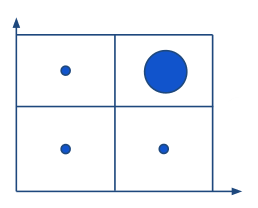
\includegraphics[height=.22\linewidth]{adh-init}
    \label{fig:adh-init}
  }
  \subfigure[Cell subdivision and computation of the sample
    alignment probability for new cells]{%
    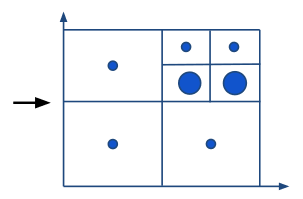
\includegraphics[height=.22\linewidth]{adh-step}
    \label{fig:adh-step}
  }
  \subfigure[Further subdivision \textcolor{red}{details}]{%
    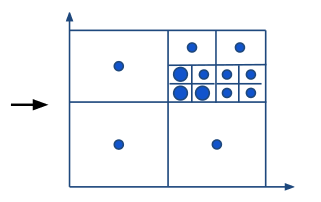
\includegraphics[height=.22\linewidth]{adh-final}
    \label{fig:adh-final}
  }
  
  \caption{Dynamic refinement of an annealed dynamic histogram. The
    grid cells devide the state space. The size of the circles
    indicates the probability for the state in the cell given the
    measurements~\cite{paper}.}
  \label{fig:adh}
\end{figure}

To build the annealed dynamic histogram, we start with a coarsely
devided state space and compute the sample alignment probability
$p(x_t|z_1,...,z_t)$ for each cell. Figure~\ref{fig:adh-init} shows an
example initialization. Then a cell is chosen to be devided into $k$
subcells as in Figure~\ref{fig:adh-step} and~\ref{fig:adh-final}. For
the new created cells, the sample alignment probability is computed
again. To compute the probabilities for the new subcells, we first
define $|c|$ as the volume of cell $c$ and $R$ as the region of cell
we chose to subdevide into subcells $c_i$. This region does not have
to be contiguous. The new probability $p(c_i)$ of subcell $c_i$ can be
computed as follows:
\begin{align}
p(c_i)
&=p(c_i\cap R)\nonumber\\
&=p(c_i|R)p(R)\nonumber\\
&=\frac{p(x_i|z_1,...,z_t)|c_i|}{\sum_{c_j\in
    R}p(x_j|z_1,...,z_t)|c_{j\mathrm{ \textcolor{red}{ not i right?}}}|}p(R)\nonumber\\
&=\eta p(x_i|z_1,...,z_t)p(R)
\end{align}
Thus, the intuitive property $\sum_{c_i\in R}p(c_i)=p(R)$
holds. $\eta$ is again used for normalization and depends only on the
the subcells in region $R$. Therefore, the probabilities of all cells
outside of $R$ are not changed.

Loosely speaking, the criteria that chooses which cells to devide in
the next step, tries to maximize the information gain. Prefered
subdevisions result in a more definite distribution of probabilities
in the subcells. In other words, the probability of the cell to devide
is condensed in a few subcells instead of uniformly distributed. 
To measure this information gain, we inspect the distribution in the
possible subcells before and after deviding. Let distribution $B$ be
currently estimated distribution in the subcells before
deviding. Because we only know the probability of the parent-cell, we
assume that this probability is equally distributed among the subcells
as illustrated in the left of Figure~\ref{fig:adh-criteria}.
\begin{figure}
  \center
  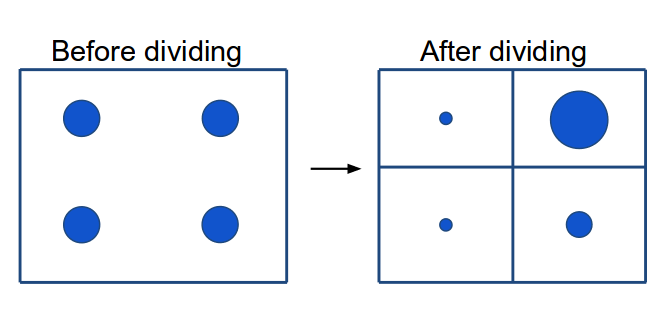
\includegraphics[width=0.55\linewidth]{devision-criteria}
  \caption{Before deviding a parent-cell we assume that its
    probability is equally distributed amoung the $k$ subcells. After
    deviding, each subcell has its own probability.~\cite{paper}.}
  \label{fig:adh-criteria}
\end{figure}
After deviding the parent-cell, each of the $k$ subcell has its own
probability and the only constraint is that the sum of the subcell
probabilities has to match the parent-cells probability $\sum_{j=1}^k p_j=P_i$. The new
distribution of probabilities amoung the subcells is called $A$ and is
a better approximation of the true posterior than $B$.

This kind of information gain can be computed with the
Kullback–Leibler divergence \textit{(KL-divergence)}~\cite{kl-divergence}. The
KL-divergence of $B$ from $A$ measures the information loss when $A$
is approximated with $B$. In our case, we can compute the
KL-divergence with
\begin{align}
  D_{KL}(A||B)=\sum_{j=1}^k p_j \mathrm{ln}\left(\frac{p_j}{P_i/k}\right)
\end{align}
where $A$ and $B$ are the distributions after and before deviding as
described before. In the mostly prefered case of a subdevision,
$p_{j'}=P_i$ for one $j'$ and $p_j=0$ for all $j\neq j'$. This is also
the case in which the KL-divergence has its maximum value
\begin{align}
  D_{KL}(A||B)=P_i \mathrm{ln}(k) \mathrm{ . }
  \label{eq:max-kl}
\end{align}
The minimum value of the KL-divergence $D_{KL}(A||B)=0$ is reached
when the probability $P_i$ of the parent-cell is uniformly devided
amoung the subcells. This is truly the minimum value because the
KL-divergence is always non-negative~\cite{kl-divergence} and in this
case there is no profit in deviding this parent-cell. With
Equation~\ref{eq:max-kl} we can derive that the maximum KL-divergence
per second is $P_i \frac{\mathrm{ln } (k)}{kt}$ where $t$ is the time
to compute a probability for a subcell with the measurement
model. Because $k$ is constant and $t$ should roughly be the same over
the whole state spave, we have to devide the cells with the highest
probability first to convert as fast as possible to the true
posterior. If we want to devide all cells that have a higher
probability than a threshold $p_{min}$, we can also devide all these
cells in each iteration, as it is done in Figure~\ref{fig:adh}. This
also yields a simple termination criteria. To maximize the the
convergence speed to the true posterior, $k$ should be chosen as small
as possible. For example if the histogram has $d$ dimensions, $k=3^d$
could be used.

\subsubsection{Annealing}
\label{sub:annealing}
With the devision of cells into k subcells and the criteria to choose
which cells to devide, we have a dynamic histogram that works in
principle. Because of the coarse resolution of the histogram,
especially at the initialization, we can not expect to find a good
alignment between the two point clouds in the current and previous
frame. The coarse resolution thus introduces an additional
error-source in the method. A solution for this problem is to include
the error resulting from the resolution as variance into the
measurement model. We increase the variance of the measurement model
Gaussian by a value $\Sigma_g$. Because the introduced error is
expected to be smaller for a better resolution, $\Sigma_g$ is
expressed as a function proportional to the resolution in the
currently inspected cell. The updated variance of the measurement
model then is $\Sigma = 2\Sigma_e+\Sigma_r+\Sigma_g$. As the
resolution improves, the term for $\Sigma_g$ decreases towards $0$ and
the variance converges against the value as before. Therefore, the
measurement model is annealed as the resolution is improved.


\subsubsection{Resulting Tracking Estimate}
\label{sub:adh-resulting}
After terminating because all cell-probabilities are below the
threshold $p_{min}$ or the computation was stopped due to real-time
restrictions, the result of the position and velocity estimation can
be returned. There are multiple possibilities what result can be
returned by the histogram. The simplest approach would be to return
the mean and variance of the distribution. An alternative would be to
return the mode of the distribution. For sophisticated planners which
would be used in an autonomous car, also the complete probability
distrubution as a density tree could be returned~\cite{density-tree}.
Using the mean of the distribution has the advantage that this would
minimize the \textit{Root-Mean-Square error (RMS error)} as shown
in~\cite{paper}. \textcolor{red}{Probabily show this?}.

% +++++++++++++++++++++++++
\section{Evaluation}
\label{sec:evaluation}
This section evaluates the tracker using the position and velocity
estimation with annealed dynamic histograms and a model which combines
cues from 3D shape, color, and motion. It presents the experiments and
results of~\cite{paper}. The main criteria of the evaluation are the
robustness, the precision, and the runtime of the proposed
method. The performance in these criteria is compared with other
widely used tracking methods for position and velocity estimation,
such as ICP and Kalman filters.

Although there are some existing evaluation methods for tracking, they
mostly are not applicable or not suitable for the autonomous driving
application. Many standard evaluation techniques are not applicable
because the method we want to evaluate only focuses on a subpart of
tracking, namely position and velocity estimation. From the tracking
evaluation techniques for tracking multiple objects, the metric called
\textit{multiple object tracking accuracy (MOTA)} can not be used
because it incorporates penailties for wrong assignments called id
switches. \textit{Multiple object detection accuracy (MODA)} considers
the amount of incorrect detections (e.g. false
positives). \textit{Multiple object detection precision (MODP)}
measures the position detection in single frames (e.g. to find the
centroid). These three metrics are not aplicable here, because the
presented method is not responsible for these problems. The metric
called \textit{multiple object tracking precision (MOTP)} would be
suitable for the method because it only evaluates the precision of the
position estimation given a correct matching~\cite{mot,mot2}. However,
the authors of the presented paper focus on measuring the
\textit{Root-Mean-Square error (RMS error)}
\begin{align}
  e_{RMS}=\sqrt{\mathbb{E}((\hat{v}_t-v_t)^2)}
\end{align}
where $\mathbb{E}$ is the mean and $\hat{v}_t-v_t$ is the velocity
tracking error. We focus here on the velocity instead of the whole
state with position and velocity because the position $x_{t,p}$ in the
state is relative to the objects position in the previous frame and
mainly used for estimating the velocity with the motion model. The
absolute position of the tracked object can easily be computed as the
centroid of the point cloud and thus has not to be evaluated here. The
RMS error is widely used and has the property to give large errors a
higher influence than many small ones have. A problem with the RMS
error, which was not mentioned by the authors of the paper, is that it
is independent of the distance to the object. Intuitively, the
tracking error for distant objects whould be higher than for close
objects because the point clouds have less measurement
points. However, the authors might have considered it in the
evaluation because the distance to the tracked object is incorporated
in the variance of the measurement model Gaussian and therefore also
in the variance of the returned tracking estimate.

To properly evaluate the performance of the tracker, a large dataset
with many different objects to track is needed, because in practise an
autonomous car has to track many different objects with different
shapes, color distributions, and motion patterns. Therefore, the
aquisition of evaluation data has to be scalable. This excludes
methods as done by~\cite{unscalable-eval} where the tracking and
tracked cars were equipped with additional sensors to measure the
positions and velocities. The authors of the paper presented in this
report propose two approaches to automatically generate test data and
evaluate the tracking with it. In both approaches, the car was driven
around and the sensor data with object detection and object assignment
was recorded. Therefore, a large amount and variety of tracked object
in the surrounding of the car is automatically recorded and the data
is taken from a environment that is close or equal to the application
environment. In the first approach which is presented in
Subsection~\ref{sub:relative-ref-frame}, the car drives in a
parking space where the tracked objects are not moving. By assuming
that the car is standing still, the tracked objects seem to be
moving and their  velocity can be tracked. The results can
be compared to the velocity calculated with the cars movement and the
distance to the tracked object. The second approach is described in
Subsection~\ref{sub:model-crispness} and utilizes a recorded dataset
from the car driving in real traffic. Using the relative positions of
the point clouds calculated by the tracker, the point clouds can be
merged to build a model of the tracked object. Then a metric is
introduced to measure the quality of the build model.

Before the tracking can be evaluated, the various parameters
introduced in the method have to be determined. This was done by using
a training dataset that is different from the test sets used
later. The training dataset was generated by recording while the car
drives past parked cars. The approach is similar to the first
evaluation approach. The most important parameters determined
in~\cite{paper} are the initial coarse resolution of $1$m for the
annealed dynamic histogram, the variance $\Sigma_g=gI$ to anneal the
measurement model, where $g$ is the cell resolution and $I$ is the
identity matrix, and $p_c=0.05$ for the color model. This results in a
low probability $p(C)$ for a color match because of many underexposed
frames and frames with lense flare.

\subsection{Relative Reference Frame}
\label{sub:relative-ref-frame}
\begin{figure}
  \center
  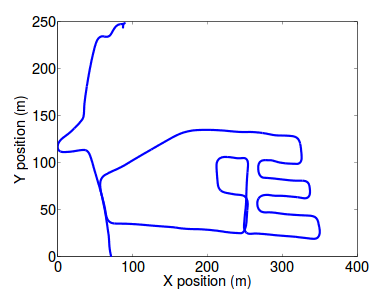
\includegraphics[width=.45\linewidth]{rel-ref-frame-path}
  \caption{Path taken by the tracking car on the parking space~\cite{paper}.}
  \label{fig:rel-ref-frame-path}
\end{figure}

In the first approach, the test data is recorded by a car driving on a
parking space. During the recording of $6.6$ minutes, about $560$ cars
were tracked. This large dataset allows a good quantitative
evaluation. The objects were tracked in a local reference frame. This
means that the tracker assumes that the recording car stands still and
the tracked objects move around it. The path of the car through the
parking space is shown in Figure~\ref{fig:rel-ref-frame-path}. Even in
this simplified scenario, many real world challenges for the tracking
are present in the dataset. Viewpoint changes, changes in occlusion
and color changes due to reflections from different viewpoints are
similar to driving in traffic. During the recording, the linear and
rotational velocity of the tracking car is logged. With this
information, the ground-truth velocity of the tracked objects can be
computed. When the car is driving just forward this is easy. When the car
is turning, the relative position of the tracked objects is used
additionally. Because of many objects beeing inside and outside the
turning circle of the car, the distribution of velocities of the
tracked objects is wider than the simple velocity distribution of the
car. These velocity distributions are plotted in
Figure~\ref{fig:rel-ref-frame-vel} and~\ref{fig:rel-ref-frame-rot}.
\begin{figure}
  \center
  \subfigure[Distribution of linear velocities]{%
    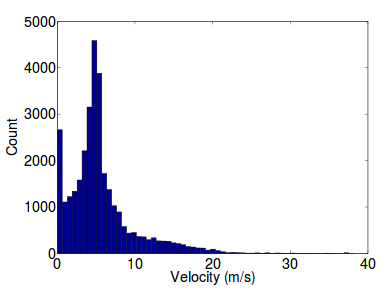
\includegraphics[height=.32\linewidth]{rel-ref-frame-vel}
    \label{fig:rel-ref-frame-vel}
  }
  \subfigure[Distribution of rotational velocities]{%
    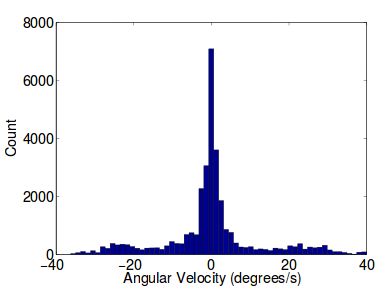
\includegraphics[height=.32\linewidth]{rel-ref-frame-rot}
    \label{fig:rel-ref-frame-rot}
  }
  \caption{Distribution of the ground-truth velocities of the tracked
    objects in the local refference frame~\cite{paper}.}
  \label{fig:rel-ref-frame}
\end{figure}

To evaluate only the position and velocity estimation part of the
tracking pipeline, some tracked objects over a number of successive
frames, called tracks, are filtered out. About $7\%$ of the tracks
were filtered out due to undersegmentation issues. Undersegmentation
occurs when multiple nearby objects are not distinguished in the
segmentation step and therefore wrongly detected as one object. These
tracks are filtered out because of the ambiguity in the ground-truth
velocity. Tracks with oversegmentation, where one object is split into
multiple peaces is not filtered out.

We now compare the performance of the proposed tracking method with
several widely used baseline methods. One the one hand, we compare the
RMS error and on the other hand the mean runtime.
Figure~\ref{fig:rms-runtime} shows the results of the
comparison. Plotted are RMS errors at different mean runtimes for the
method presented in this report as well as four other baseline methods.

The first baseline method we use for comparison is a Kalman filter that
uses only the centroid of point cloud in a frame in its measurement
model. This method is widely used because of the easy implementation
and the fast computation. As shown in Figure~\ref{fig:rms-runtime} the
Kalman filter is extremely fast with a computational time below $0.1$
milliseconds. This was expected because the Kalman filter only uses
the centroid instead of aligning two point clouds. The RMS error is
$0.78 \mathrm{~m/s}$ and shows that the Kalman filter is not very
accurate. For the Kalman filter, there is only a single mean runtime
because the Kalman filter only has a single computation step and no
dynamic improvement steps.

\begin{figure}
  \center
  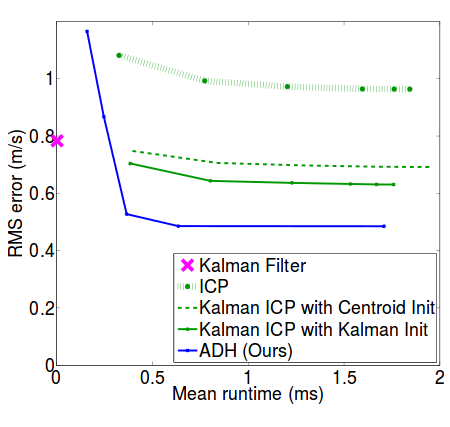
\includegraphics[width=.45\linewidth]{rms-vs-runtime}
  \caption{Comparison of the proposed method with annealed dynamic
    histograms with other baseline methods. Plotted is the RMS error
    for different runtimes of the algorithm~\cite{paper}.}
  \label{fig:rms-runtime}
\end{figure}

Furthermore, we analyze the performance of ICP in different
variants. These variants differ in the initialization of ICP and
wheather they are used as a measurement model in for Kalman
filter. The basic point-to-point ICP algorithm is described
in~\cite{icp-basic} and uses the centroid of the point clouds to align
as initialization. The algorithm was run with up to $100$ incremental
alignment iterations. The RMS error with different mean runtimes is
shown in Figure~\ref{fig:rms-runtime} and is about
$1\mathrm{~m/s}$. This is $23\%$ worse than the RMS error of a simple
Kalman filter and therefore no good tracking performance. This bad
performance in comparison to the Kalman filter is caused by the
missing motion model which is important for robust tracking. Without a
motion model, only the last two frames can be used to estimate the
velocity of the tracked object. Therefore, a single incorrect
alignment as, for example, show in Figure~\ref{fig:icp} significantly
impacts the tracking error. A Kalman filter with its motion model
can refine the result of many more previous alignments into one
Gaussian distribution and can compensate wrong alignments because the
ceartainty of a measurement can be considered as variance when feeding
the measurement into the Kalman filter. 

By combining the Kalman filter and ICP into one method, the drawbacks
of both methods can be removed. ICP can be used as measurement model
to align the point clouds in successive frames what removes the
information loss in the basic Kalman filter that only uses the
centroid. The result can be used in the motion model of the Kalman
filter. 
\subsection{Model Crispness}
\label{sub:model-crispness}

% +++++++++++++++++++++++++
\section{Conclusion}
\label{sec:conclusion}


% =========================================================================
\bibliographystyle{alpha}
\bibliography{seminar_report}

% =========================================================================

\end{document}
